
\documentclass[12pt,a4paper]{report}

\usepackage[a4paper,margin=1in,headheight=15pt]{geometry}
\usepackage[T1]{fontenc}
\usepackage{lmodern}
\usepackage{setspace}
\usepackage{graphicx}
\usepackage{float}
\usepackage{booktabs}
\usepackage{longtable}
\usepackage{array}
\usepackage{tabularx}
\usepackage{enumitem}
\usepackage{fancyhdr}
\usepackage{titlesec}
\usepackage{xcolor}
\usepackage{hyperref}
\usepackage{tikz}
\usetikzlibrary{arrows.meta,positioning,shapes.geometric,shapes.multipart,fit,calc}
\usepackage{listings}
\usepackage{caption}

\definecolor{tietblue}{RGB}{25,76,135}
\definecolor{lightblue}{RGB}{226,239,252}
\definecolor{lightgray}{RGB}{245,246,248}
\hypersetup{colorlinks=true,linkcolor=tietblue,urlcolor=tietblue,citecolor=tietblue}
\setstretch{1.18}
\setlist[itemize]{leftmargin=1.5em,itemsep=3pt}
\setlist[enumerate]{leftmargin=1.7em,itemsep=3pt}
\pagestyle{fancy}
\fancyhf{}
\lhead{\small UCS503 -- Software Engineering Project}
\rhead{\small AI-Enabled Smart Library Management System}
\cfoot{\thepage}
\titleformat{\chapter}[display]{\normalfont\bfseries\Huge\color{tietblue}}{\chaptername\ \thechapter}{10pt}{\Huge}
\titleformat{\section}{\normalfont\Large\bfseries\color{tietblue}}{\thesection}{0.7em}{}
\titleformat{\subsection}{\normalfont\large\bfseries}{\thesubsection}{0.7em}{}

\newcommand{\diagram}[3]{%
\begin{figure}[H]\centering
\IfFileExists{#1}{\includegraphics[width=#2\textwidth,height=0.72\textheight,keepaspectratio]{#1}}%
{\fbox{\parbox[c][4.2cm][c]{0.82\textwidth}{\centering
\textbf{Diagram file not found}\\[4pt]\texttt{#1}\\[4pt]
Place the corresponding image at this path to display it.}}}%
\caption{#3}\end{figure}}

\begin{document}

% ---------------- COVER PAGE ----------------
\begin{titlepage}
\thispagestyle{empty}
\begin{center}
\vspace*{0.4cm}
{\large\bfseries UCS503 -- Software Engineering Lab}\\[1.2cm]
{\Large\bfseries AI-ENABLED SMART LIBRARY MANAGEMENT AND RESOURCE RECOMMENDATION SYSTEM}\\[0.7cm]
{\large\bfseries UCS503 Software Engineering Project Report}\\[0.35cm]
{\large\bfseries END-SEMESTER EVALUATION}\\[1.3cm]
{\large\bfseries Submitted by:}\\[0.45cm]
{\large (1024160010) Arnav Agarwal}\\[0.2cm]
{\large (1024160135) Aradhya Goyal}\\[0.2cm]
{\large (1024160025) Amanjot Kaur Sidhu}\\[0.55cm]
{\large B.E. Third Year, Computer Science and Engineering}\\[0.25cm]
{\large Group No.: To be confirmed}\\[1.0cm]
{\large\bfseries Submitted to:}\\[0.35cm]
{\large Dr. Jeelani Asif}\\[1.0cm]
\vfill
{\Large\bfseries Computer Science and Engineering Department}\\[0.25cm]
{\Large\bfseries Thapar Institute of Engineering and Technology}\\
{\large Patiala}\\[0.35cm]
{\large November 2026}
\end{center}
\end{titlepage}

\pagenumbering{roman}
\chapter*{Declaration}
We declare that this report presents the analysis, design, documentation, and prototype work carried out for the UCS503 Software Engineering Project titled \textit{AI-Enabled Smart Library Management and Resource Recommendation System}. The report distinguishes design objectives and prepared test cases from functionality whose execution has not yet been verified. Any implementation status stated in this report is based on the project information and progress records available at the time of preparation.

\vspace{1.5cm}
\noindent Arnav Agarwal \hfill Aradhya Goyal\\[1.0cm]
\noindent Amanjot Kaur Sidhu

\chapter*{Acknowledgement}
We express our sincere gratitude to our faculty instructor, Dr. Jeelani Asif, for guidance and feedback during the development of this project. We also acknowledge the support and collaboration of our team members throughout project selection, analysis, design, documentation, and prototype preparation.

\chapter*{Abstract}
The AI-Enabled Smart Library Management and Resource Recommendation System is proposed as a web-based platform that combines conventional library operations with controlled AI-assisted resource discovery. The system is designed around a three-tier architecture consisting of a React-based web interface, a FastAPI backend, and a MySQL relational database, with a controlled AI agent layer.

The proposed platform covers student and resource record management, book issue and return transactions, due-date and fine tracking, natural-language resource discovery, bulk record onboarding, and overdue notifications. Three specialized agents are defined: the Library Intelligence Agent for interpreting natural-language resource requests and producing availability-aware results; the Record Onboarding Agent for validating bulk records and identifying possible duplicates; and the Library Monitoring Agent for overdue monitoring, fine workflows, and library activity analysis.

This report documents the project selection, requirements analysis, system models, software design, prototype direction, and prepared functional test cases. The supplied test workbook contains test scenarios whose execution status is recorded as \textit{Not run}; therefore, this report does not claim that those tests have passed. The project emphasizes incremental engineering, controlled database access, measurable evaluation, and clear separation between AI-assisted interpretation and deterministic transaction processing.

\tableofcontents
\listoffigures
\listoftables
\clearpage
\pagenumbering{arabic}

% ---------------- 1 PROJECT SELECTION ----------------
\chapter{Project Selection Phase}

\section{Software Bid}
The proposed software is an academic library-management application intended to improve the discoverability and administration of library resources. The project is scoped as a student-developed software prototype for the UCS503 course rather than a commercial procurement bid. Its proposed value is the consolidation of routine library workflows with controlled assistance for natural-language discovery and administrative automation.

\subsection{Proposed Scope}
The planned scope includes:
\begin{itemize}
\item maintaining student/member and library resource records;
\item supporting book issue and return transactions;
\item tracking due dates, overdue records, and fines;
\item allowing direct catalogue lookup and natural-language discovery;
\item validating bulk student/resource records and identifying duplicates;
\item creating overdue notification entries; and
\item presenting useful circulation and library activity information to administrators.
\end{itemize}

\subsection{Expected Benefits}
The system is intended to reduce repetitive manual work, make catalogue discovery more accessible, improve visibility into circulation status, and provide a structured foundation for future library automation. The expected benefits are design objectives and are not represented as measured outcomes at this stage.

\section{Project Overview}
The AI-Enabled Smart Library Management and Resource Recommendation System is a web-based library platform. It combines deterministic library operations with a constrained AI layer. Students can search for a specific book or describe the subject and type of material they need. Librarians/admin users can manage records and circulation workflows.

\subsection{Project Objectives}
\begin{enumerate}
\item Develop a centralized digital library-management platform.
\item Support direct catalogue lookup for students who know a title or other identifying information.
\item Enable natural-language resource discovery for open-ended recommendation requests.
\item Provide availability-aware search results based on current circulation data.
\item Support bulk student and resource record onboarding.
\item Detect duplicate or potentially duplicate records before insertion.
\item Monitor overdue loans and calculate fines using deterministic business rules.
\item Create notification entries for affected students.
\item Maintain controlled and auditable interaction between AI services and the database.
\end{enumerate}

\subsection{Project Selection Rationale}
The library domain provides a bounded and practical problem space with identifiable users, records, transactions, and measurable workflows. The project can deliver value incrementally: core catalogue and circulation functionality can be developed independently of AI-assisted discovery. Mature technologies such as React, FastAPI, MySQL, Pydantic, and established language-model APIs are available, reducing the need for novel research.

% ---------------- 2 ANALYSIS ----------------
\chapter{Analysis Phase}

\section{System Stakeholders}
\begin{itemize}
\item \textbf{Student:} searches the catalogue, requests resources, views loan/fine information, and receives notifications.
\item \textbf{Librarian:} manages catalogue records, performs circulation operations, and reviews administrative information.
\item \textbf{Administrator:} manages student/resource onboarding and system configuration.
\item \textbf{Library Intelligence Agent:} interprets natural-language requests and returns structured search intent to backend services.
\item \textbf{Record Onboarding Agent:} validates batch records and identifies possible duplicates.
\item \textbf{Library Monitoring Agent:} supports overdue monitoring and notification workflows.
\end{itemize}

\section{Use Cases}

\subsection{Use-Case Diagram}
\diagram{docs/Diagrams/Use Case Diagram/Use Case Diagram.png}{0.88}{Use Case Diagram of the Smart Library Management System.}

\subsection{Use-Case Templates}
\subsubsection{UC-01: Search Library Resources}
\textbf{Primary actor:} Student.\\
\textbf{Preconditions:} The catalogue is available. The student can access the search interface.\\
\textbf{Main flow:}
\begin{enumerate}
\item The student enters a title, author, ISBN, subject, or natural-language request.
\item The interface sends the request to the backend.
\item For a direct lookup, the backend performs catalogue matching. For a recommendation request, the Library Intelligence Agent extracts intent and keywords.
\item The backend retrieves matching catalogue records and calculates current availability.
\item Ranked results and availability information are returned to the student.
\end{enumerate}
\textbf{Alternate flow:} If no matching resource is found, the system displays an appropriate no-results response.\\
\textbf{Postcondition:} Search activity may be recorded for later analysis.

\subsubsection{UC-02: Issue a Resource}
\textbf{Primary actor:} Librarian.\\
\textbf{Preconditions:} The student is eligible to borrow and the requested copy is available.\\
\textbf{Main flow:}
\begin{enumerate}
\item The librarian selects the student and resource.
\item The backend validates eligibility and availability.
\item The system creates an issue transaction and assigns issue and due dates.
\item The catalogue/circulation state is updated.
\item A confirmation is displayed.
\end{enumerate}
\textbf{Alternate flow:} The request is rejected if the resource is unavailable or the borrowing limit is reached.\\
\textbf{Postcondition:} An active issue record exists for the student and resource.

\subsubsection{UC-03: Return a Resource}
\textbf{Primary actor:} Librarian.\\
\textbf{Preconditions:} An active issue record exists.\\
\textbf{Main flow:}
\begin{enumerate}
\item The librarian locates the active issue.
\item The backend records the return date and updates the issue status.
\item The resource becomes available for future circulation.
\item If the resource is overdue, the fine workflow calculates the applicable amount.
\item The system displays return confirmation.
\end{enumerate}
\textbf{Postcondition:} The issue record is closed and circulation data is updated.

\subsubsection{UC-04: Bulk Record Onboarding}
\textbf{Primary actor:} Administrator.\\
\textbf{Preconditions:} The administrator is authenticated and has onboarding permission.\\
\textbf{Main flow:}
\begin{enumerate}
\item The administrator submits a structured batch of student or resource records.
\item The onboarding service validates required fields and formats.
\item Duplicate identifiers and potential fuzzy matches are flagged.
\item Valid records are inserted through a controlled backend transaction.
\item The system returns an import summary showing accepted and flagged records.
\end{enumerate}
\textbf{Postcondition:} Valid records are stored; flagged records are not silently inserted as new entities.

\subsubsection{UC-05: Monitor Overdue Loans}
\textbf{Primary actor:} Library Monitoring Agent / scheduled backend worker.\\
\textbf{Preconditions:} Active issue records and due dates are available.\\
\textbf{Main flow:}
\begin{enumerate}
\item The monitoring process identifies active loans past their due date.
\item The backend calculates overdue days and the applicable fine.
\item Fine records are created or updated according to the defined business rules.
\item A notification entry is queued for the affected student.
\end{enumerate}
\textbf{Postcondition:} Overdue and fine information is updated and a student notification is queued.

\section{Activity Diagram and Swimlane Diagrams}
The activity/swimlane model represents the interactions among the student, web interface, backend, Library Intelligence Agent, MySQL database, and librarian/notification roles. It focuses on the intelligent discovery and borrowing workflow.

\diagram{docs/Diagrams/Swimlane Diagram/SwimLane_Diagram.png}{0.95}{Activity / Swimlane Diagram for intelligent resource discovery and borrowing.}

\section{Data Flow Diagrams (DFDs)}
The DFDs represent information exchange between students, librarians, backend processes, AI agents, and persistent data stores.

\subsection{DFD Level 0 -- Context Diagram}
\diagram{docs/Diagrams/Data Flow Diagrams/DFD_Level0.png}{0.88}{Level 0 Context Data Flow Diagram.}

\subsection{DFD Level 1 -- System DFD}
\diagram{docs/Diagrams/Data Flow Diagrams/DFD_Level1.png}{0.90}{Level 1 Data Flow Diagram showing the major system processes.}

\subsection{DFD Level 2 -- Intelligent Search}
\diagram{docs/Diagrams/Data Flow Diagrams/Level_2_DFD.png}{0.90}{Level 2 Data Flow Diagram for intelligent resource search.}

\section{Software Requirement Specification in IEEE Format}

\subsection{Introduction}
\textbf{Purpose:} This section records the principal requirements for the Smart Library Management System.\\
\textbf{Scope:} The system supports library catalogue management, student records, circulation, fine tracking, resource discovery, bulk onboarding, and overdue notification workflows.\\
\textbf{Users:} Students, librarians, and administrators.

\subsection{Overall Description}
The system is designed as a three-tier web application. The frontend communicates with backend REST endpoints. The backend performs authorization, validation, business logic, and database access. AI components provide constrained interpretation and recommendation assistance but do not receive unrestricted database write access.

\subsection{Functional Requirements}
\begin{longtable}{p{1.5cm}p{11.5cm}}
\toprule
\textbf{ID} & \textbf{Requirement}\\
\midrule
FR-01 & The system shall allow authorized users to access role-appropriate library functions.\\
FR-02 & The system shall maintain student/member records.\\
FR-03 & The system shall maintain book/resource catalogue records.\\
FR-04 & The system shall support direct catalogue search using identifying terms such as title or ISBN.\\
FR-05 & The system shall support natural-language resource requests through the Library Intelligence Agent.\\
FR-06 & The system shall return availability based on current circulation records.\\
FR-07 & The system shall create issue records only after eligibility and availability checks.\\
FR-08 & The system shall record returns and update circulation status.\\
FR-09 & The system shall calculate overdue days and fines using deterministic backend rules.\\
FR-10 & The system shall queue overdue notifications for the affected student.\\
FR-11 & The system shall validate batch records and flag duplicate identifiers or likely duplicates.\\
FR-12 & The system shall maintain search activity records where configured for demand analysis.\\
\bottomrule
\end{longtable}

\subsection{Non-Functional Requirements}
\begin{itemize}
\item \textbf{Performance:} The proposal target for resource discovery is no more than 10 seconds; median API response target is no more than 500 ms under the defined evaluation setup.
\item \textbf{Reliability:} Circulation and fine updates should use database transactions to avoid partial updates.
\item \textbf{Security:} Database access should use parameterized queries/ORM operations and role-based authorization.
\item \textbf{AI safety:} AI outputs must be validated against structured schemas. AI agents must not execute unrestricted SQL or perform direct database writes.
\item \textbf{Maintainability:} Frontend, backend, database models, and agent modules should remain modular.
\item \textbf{Usability:} Students should be able to perform direct lookup without invoking unnecessary recommendation processing.
\end{itemize}

\subsection{External Interface Requirements}
The proposed student/admin interface is web-based. Backend services expose REST endpoints. The relational persistence layer uses MySQL. The AI layer communicates through controlled application services and validated structured outputs.

\section{User Stories and Story Cards}
\begin{longtable}{p{1.2cm}p{3cm}p{7.7cm}}
\toprule
\textbf{ID} & \textbf{Role} & \textbf{User story}\\
\midrule
US-01 & Student & As a student, I want to search by exact title or ISBN so that I can quickly locate a known book.\\
US-02 & Student & As a student, I want to describe a subject or learning goal in natural language so that I can receive relevant recommendations.\\
US-03 & Student & As a student, I want to see availability so that I know whether a resource can be borrowed.\\
US-04 & Student & As a student, I want to view my active loans and outstanding fines so that I can manage my borrowing.\\
US-05 & Librarian & As a librarian, I want to issue and return resources so that circulation records remain accurate.\\
US-06 & Administrator & As an administrator, I want to import student records in batches so that onboarding is efficient.\\
US-07 & Administrator & As an administrator, I want duplicate records flagged before insertion so that data quality is preserved.\\
US-08 & Student & As a student, I want overdue notifications so that I am informed about pending returns.\\
\bottomrule
\end{longtable}

% ---------------- 3 DESIGN ----------------
\chapter{Design Phase}

\section{System Architecture}
The system follows a modular three-tier design with a controlled AI agent layer:
\begin{enumerate}
\item \textbf{Presentation tier:} React web interface for student and administrative workflows.
\item \textbf{Application tier:} FastAPI backend exposing REST endpoints, validating requests, enforcing permissions, and coordinating business services.
\item \textbf{Data tier:} MySQL relational database containing students, employees, assets/books, issue details, fines, notifications, and search logs.
\item \textbf{AI agent layer:} Library Intelligence, Record Onboarding, and Library Monitoring modules operating through controlled backend interfaces.
\end{enumerate}

\section{Entity Relationship Diagram}
\diagram{docs/Diagrams/ER Diagram/ER_Diagram.png}{0.95}{Entity Relationship Diagram of the Smart Library Management System.}

\subsection{Principal Entities}
\begin{longtable}{p{3.3cm}p{9cm}}
\toprule
\textbf{Entity} & \textbf{Purpose}\\
\midrule
STUDENTS & Stores student identifiers, names, department, year, contact details, and status.\\
EMPLOYEE & Stores librarian/employee identifiers, names, roles, and contact information.\\
ASSETS & Stores library asset identifiers, names, types, and status.\\
BOOKS & Stores book-specific details such as title, ISBN, publisher, category, and total copies.\\
ISSUING\_DETAILS & Records issue, due, and return dates and the student, employee, and asset involved.\\
FINES & Stores fine records associated with issue transactions.\\
NOTIFICATION\_QUEUE & Stores notifications addressed to students, including message type and delivery status.\\
SEARCH\_DEMAND\_LOGS & Records student search queries and extracted categories for later analysis.\\
\bottomrule
\end{longtable}

\subsection{Normalisation Considerations}
The data model separates student, employee, asset, book, circulation, fine, and notification information into related entities. This reduces repeated storage of student and book details in transaction records. Primary keys identify records, while foreign keys maintain referential integrity. Book-specific attributes are separated from general asset attributes so that the asset catalogue can be extended if additional resource types are introduced. Search logs and notification records are stored separately because they have independent lifecycles and multiple records may be associated with one student.

\section{Class Diagrams}
The class model describes the main application objects, their attributes, operations, and relationships. The available class diagram should be placed below. A second significant class-diagram case is listed as a design extension because a second finalized class diagram was not included in the supplied materials.

\diagram{docs/Diagrams/Class Diagram/ClassDiagram.png}{0.95}{Class Diagram of the Smart Library Management System.}

\subsection{Principal Classes}
\begin{itemize}
\item \textbf{Student:} roll number, name, department, year, email, phone number, and status; operations include viewing loans and searching resources.
\item \textbf{Book:} asset identifier, title, ISBN, publisher, category, and total copies; operations include catalogue lookup and availability retrieval.
\item \textbf{Issue:} issue identifier, asset, student, employee, issue date, due date, return date, and status; operations include issue and return processing.
\item \textbf{Fine:} fine identifier, issue identifier, days late, amount, paid status, and payment date; operations include fine calculation and payment-status update.
\item \textbf{Notification:} notification identifier, student, message, type, status, and creation timestamp; operations include queueing and delivery-state recording.
\item \textbf{LibraryIntelligenceAgent:} interprets natural-language requests and returns structured search intent.
\item \textbf{RecordOnboardingAgent:} validates incoming records and flags possible duplicates.
\item \textbf{LibraryMonitoringAgent:} coordinates overdue scanning and notification generation.
\end{itemize}

\section{Sequence Diagrams}
The sequence diagram models interactions between the student, web interface, backend API, Library Intelligence Agent, and MySQL database across search, issue, overdue monitoring, and return processes.

\diagram{docs/Diagrams/Sequence Diagram/SequenceDiagram.png}{0.95}{Sequence Diagram for major library management workflows.}

\subsection{Second Significant Sequence Case: Bulk Onboarding}
\begin{enumerate}
\item Administrator submits a batch of student/resource records through the web interface.
\item Backend validates the request structure and required fields.
\item Record Onboarding Agent checks identifiers and potential duplicates.
\item Backend inserts accepted records in a controlled transaction.
\item The interface displays accepted and flagged record counts.
\end{enumerate}

\section{Collaboration Diagrams}
A collaboration/communication diagram emphasizes the participating objects and their links. The following interaction is specified as the first design case; a formal diagram image can be added when produced.

\subsection{Case 1: Intelligent Resource Search}
Objects: Student, Search UI, Search Controller, Library Intelligence Agent, Catalogue Repository, and Availability Service. The Student sends a query to the Search UI; the UI invokes the Search Controller; the controller optionally invokes the agent for natural-language interpretation; the repository retrieves matching books; the Availability Service checks active issues; and ranked results are returned to the student.

\subsection{Case 2: Issue and Return Processing}
Objects: Librarian UI, Circulation Controller, Student Repository, Catalogue Repository, Issue Repository, and Fine Service. The controller validates the student and copy, creates or closes the issue record transactionally, invokes fine calculation when applicable, and returns the operation result to the UI.

\section{State Chart Diagrams}
\subsection{Case 1: Book Copy State}
A book copy may move through the following states:
\begin{center}
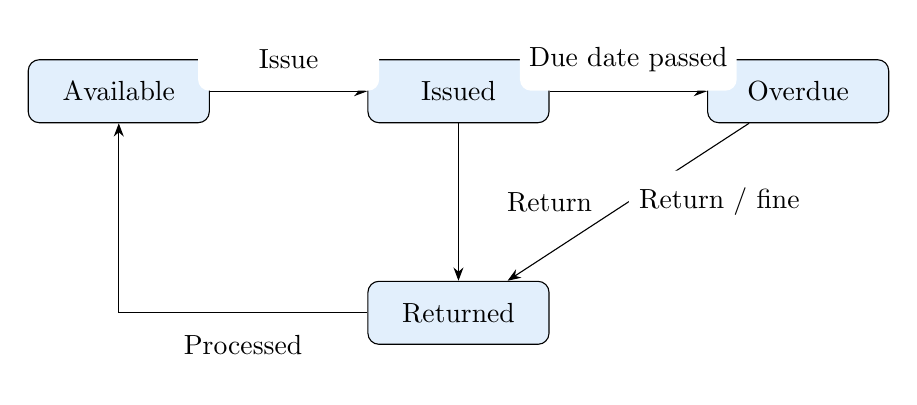
\begin{tikzpicture}[node distance=2.0cm,>=Stealth, every node/.style={draw,rounded corners,fill=lightblue,minimum width=2.3cm,minimum height=0.8cm,align=center}]
\node (available) {Available};
\node[right=of available] (issued) {Issued};
\node[right=of issued] (overdue) {Overdue};
\node[below=of issued] (returned) {Returned};
\draw[->] (available) -- node[above,draw=none,fill=white]{Issue} (issued);
\draw[->] (issued) -- node[above,draw=none,fill=white]{Due date passed} (overdue);
\draw[->] (issued) -- node[right,draw=none,fill=white]{Return} (returned);
\draw[->] (overdue) -- node[right,draw=none,fill=white]{Return / fine} (returned);
\draw[->] (returned) -| node[pos=0.25,below,draw=none,fill=white]{Processed} (available);
\end{tikzpicture}
\end{center}

\subsection{Case 2: Issue Transaction State}
An issue transaction progresses from \textit{Requested} to \textit{Validated}. If the student and copy satisfy the circulation rules, it becomes \textit{Active}. It may transition to \textit{Overdue} when the due date passes, and then to \textit{Returned} when the resource is returned. A request that fails validation is \textit{Rejected}. Fine payment is tracked as a related financial status rather than changing the physical availability state of the book.

% ---------------- 4 IMPLEMENTATION ----------------
\chapter{Implementation}

\section{Technology Stack}
\begin{longtable}{p{3.2cm}p{9cm}}
\toprule
\textbf{Layer} & \textbf{Technology / design choice}\\
\midrule
Frontend & React web application\\
Backend & FastAPI with Python 3.11+\\
Database & MySQL\\
Request validation & Pydantic\\
AI integration & LangChain / OpenAI API as proposed agent integration\\
API style & REST endpoints\\
Version control & Git and GitHub\\
Documentation & MkDocs Material and GitHub Pages\\
Automation & GitHub Actions for documentation deployment\\
\bottomrule
\end{longtable}

\section{Backend API Design}
The project API design includes the following endpoints. Their presence in the design does not by itself establish that each endpoint has been deployed or passed integration testing.

\begin{longtable}{p{2cm}p{5.5cm}p{4.7cm}}
\toprule
\textbf{Method} & \textbf{Endpoint} & \textbf{Purpose}\\
\midrule
POST & \texttt{/api/search/intelligent} & Natural-language resource search and recommendations.\\
POST & \texttt{/api/ingestion/sync} & Bulk student/resource record ingestion.\\
GET & \texttt{/api/circulation/fines/\{student\_id\}} & Retrieve student fine information.\\
POST & \texttt{/api/cron/monitor-overdues} & Trigger overdue monitoring.\\
\bottomrule
\end{longtable}

\section{Database Design}
The database design uses MySQL and separates core entities from transaction and activity records. The main tables are STUDENTS, EMPLOYEE, ASSETS, BOOKS, ISSUING\_DETAILS, FINES, NOTIFICATION\_QUEUE, and SEARCH\_DEMAND\_LOGS. Foreign-key relationships are used to connect issue records to students, employees, and assets; fines to issue records; and notification/search-log records to students.

\section{Component Diagram}
The component view should show the web client, REST API, authentication/validation services, circulation services, catalogue/search services, AI agent modules, and MySQL persistence.

\begin{center}
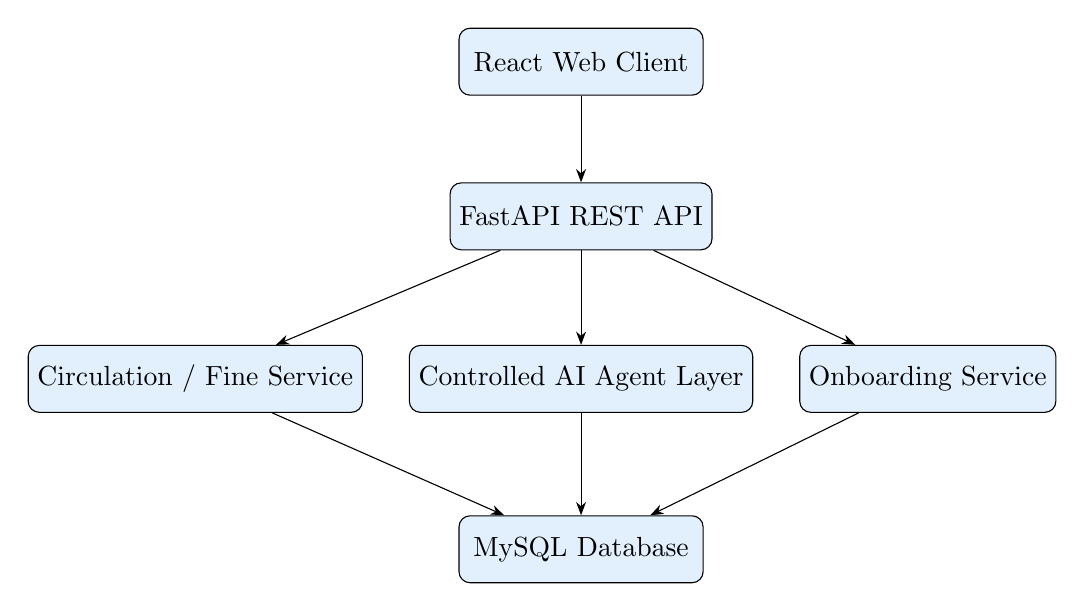
\begin{tikzpicture}[>=Stealth,node distance=1.1cm,
box/.style={draw,rounded corners,fill=lightblue,minimum width=3.1cm,minimum height=0.85cm,align=center}]
\node[box] (ui) {React Web Client};
\node[box,below=of ui] (api) {FastAPI REST API};
\node[box,below left=1.2cm and 1.1cm of api] (circulation) {Circulation / Fine Service};
\node[box,below=1.2cm of api] (agents) {Controlled AI Agent Layer};
\node[box,below right=1.2cm and 1.1cm of api] (onboard) {Onboarding Service};
\node[box,below=1.3cm of agents] (db) {MySQL Database};
\draw[->] (ui)--(api);
\draw[->] (api)--(circulation);
\draw[->] (api)--(agents);
\draw[->] (api)--(onboard);
\draw[->] (circulation)--(db);
\draw[->] (agents)--(db);
\draw[->] (onboard)--(db);
\end{tikzpicture}
\end{center}
\captionof{figure}{Logical component diagram of the proposed system.}

\section{Deployment Diagram}
The deployment view represents the logical deployment arrangement. The actual hosting provider and production topology were not supplied; therefore, this is a logical deployment model rather than evidence of a completed production deployment.

\begin{center}
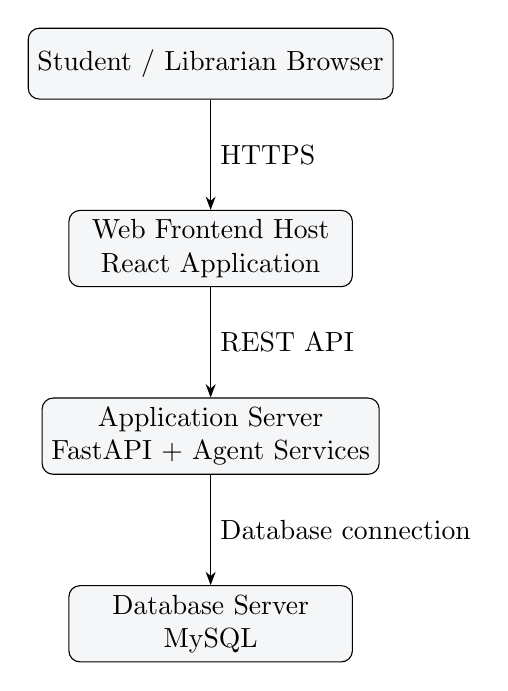
\begin{tikzpicture}[>=Stealth,node distance=1.4cm,
box/.style={draw,rounded corners,fill=lightgray,minimum width=3.6cm,minimum height=0.9cm,align=center}]
\node[box] (browser) {Student / Librarian Browser};
\node[box,below=of browser] (web) {Web Frontend Host\\React Application};
\node[box,below=of web] (server) {Application Server\\FastAPI + Agent Services};
\node[box,below=of server] (mysql) {Database Server\\MySQL};
\draw[->] (browser)--node[right,draw=none]{HTTPS}(web);
\draw[->] (web)--node[right,draw=none]{REST API}(server);
\draw[->] (server)--node[right,draw=none]{Database connection}(mysql);
\end{tikzpicture}
\end{center}
\captionof{figure}{Logical deployment diagram.}

\section{Documentation and Repository Infrastructure}
The project documentation was organized using MkDocs Material. The documentation website includes the project overview, architecture, installation guidance, criteria for project selection, and supporting diagrams. GitHub Actions was enabled for automated documentation deployment to GitHub Pages. A concise repository README was also prepared to explain the project, architecture, technology stack, structure, and key workflows.

\section{Implementation Screenshots}
Actual application screenshots were not included in the materials available for this report. Insert verified screenshots in this section when available. Documentation screenshots or design diagrams should not be presented as proof of a running application.

\begin{figure}[H]\centering
\fbox{\parbox[c][4cm][c]{0.85\textwidth}{\centering Insert verified student dashboard screenshot here.}}
\caption{Student interface screenshot -- to be added.}
\end{figure}
\begin{figure}[H]\centering
\fbox{\parbox[c][4cm][c]{0.85\textwidth}{\centering Insert verified librarian/admin dashboard screenshot here.}}
\caption{Librarian/admin interface screenshot -- to be added.}
\end{figure}

% ---------------- 5 TESTING ----------------
\chapter{Testing}

\section{Test Plan}

\subsection{Purpose}
The test plan defines how the principal library workflows should be verified. The supplied workbook contains prepared test scenarios and expected results. All recorded execution statuses in the workbook are \textit{Not run}; the cases are therefore presented as test specifications, not completed test evidence.

\subsection{Scope}
Testing is planned for:
\begin{itemize}
\item book issue eligibility and copy availability;
\item return processing and fine handling;
\item direct title lookup and natural-language recommendation routing;
\item bulk student record onboarding and duplicate detection;
\item overdue identification, fine calculation, and notification queue creation; and
\item high-demand/low-availability analysis.
\end{itemize}

\subsection{Test Approach}
Positive tests verify valid operations. Negative tests verify rejection of invalid operations. Boundary tests verify behaviour at limits, such as the maximum permitted number of active loans. Database checks should be performed after each transaction to verify persistence and consistency. Search tests should inspect both returned results and the corresponding search log where applicable.

\subsection{Test Environment}
The workbook does not specify a completed execution environment or execution date. Before execution, record the application build/version, database version, test environment, test date, and tester. Test identifiers and sample data should be isolated from production/student data.

\section{Test Cases}
The following cases are taken from the supplied test workbook. The status is reproduced as \textit{Not run}.

\small
\begin{longtable}{p{1.55cm}p{2.5cm}p{5.2cm}p{2.1cm}}
\toprule
\textbf{Test ID} & \textbf{Module} & \textbf{Scenario / expected outcome} & \textbf{Status}\\
\midrule
LMS-ISSUE-001 & Issue Book & Issue an available book to an eligible member. A single active loan should be created and available copies should decrease by one. & Not run\\
LMS-ISSUE-002 & Issue Book & Reject an issue when the member already has three active loans. No new loan should be created and availability should remain unchanged. & Not run\\
LMS-ISSUE-003 & Issue Book & Allow the third loan when the member currently has two active loans and the copy is available. & Not run\\
TC-01A & Circulation / Issue & Verify successful issue of an available resource and creation of an issue record with issue and due dates. & Not run\\
TC-01B & Circulation / Return & Return a resource on or before its due date; update the issue status and availability without generating a fine. & Not run\\
TC-02A & Intelligent Search & Interpret a natural-language machine-learning request, return relevant available resources, and log the query/category. & Not run\\
TC-02B & Search Routing & Distinguish an exact-title lookup from an open-ended recommendation request; avoid recommendation generation for direct title lookup. & Not run\\
TC-03 & Record Onboarding & Import a batch containing two new student records and one duplicate roll number; accept two and flag one duplicate. & Not run\\
TC-04A & Fine Workflow & Identify a loan five days overdue at ₹5/day and create/update a ₹25 fine record with a notification queue entry. & Not run\\
TC-04B & Demand Analysis & Identify a frequently requested resource with low stock and produce an acquisition recommendation for administrator review. & Not run\\
\bottomrule
\caption{Prepared functional test cases from the supplied workbook.}
\end{longtable}
\normalsize

\section{Test Reports by Peers}
No completed peer test reports or signed peer feedback were supplied with the current materials. This section is reserved for recording peer tester name, test case ID, execution date, actual result, pass/fail status, defect reference, and comments.

\begin{longtable}{p{2.5cm}p{2cm}p{2cm}p{2cm}p{3cm}}
\toprule
\textbf{Peer tester} & \textbf{Test ID} & \textbf{Date} & \textbf{Result} & \textbf{Remarks / defect}\\
\midrule
To be recorded & -- & -- & Not executed & Peer execution evidence not supplied.\\
\bottomrule
\caption{Peer testing record template.}
\end{longtable}

\section{Evaluation Metrics}
The proposal defines the following targets for evaluation. They are targets, not measured results.

\begin{longtable}{p{6cm}p{3cm}p{3cm}}
\toprule
\textbf{Metric} & \textbf{Target} & \textbf{Evidence status}\\
\midrule
Resource discovery time & $\leq 10$ seconds & Not measured\\
Duplicate detection precision & $\geq 90\%$ & Not measured\\
Overdue detection coverage & $\geq 99\%$ & Not measured\\
Recommendation accuracy & $\geq 90\%$ & Not measured\\
Median API response time & $\leq 500$ ms & Not measured\\
Automated test coverage & $\geq 70\%$ & Not measured\\
\bottomrule
\caption{Proposed evaluation targets and current evidence status.}
\end{longtable}

% ---------------- PROJECT SCHEDULE ----------------
\chapter{Project Schedule and Progress}

\section{Gantt Chart Summary}
The supplied Gantt workbook records project tasks from the initial project selection and proposal work through modelling, documentation infrastructure, diagrams, frontend development, and test-case preparation. The chart records the following selected milestones:

\begin{longtable}{p{7.5cm}p{2.3cm}p{2.3cm}p{1.2cm}}
\toprule
\textbf{Task} & \textbf{Start} & \textbf{End} & \textbf{Progress}\\
\midrule
Problem identification and conventional CRUD limitations research & 08 Jun 2026* & 08 Jun 2026* & 100\%\\
Multi-agent architecture and scope definition & 05 Aug 2026 & 09 Aug 2026 & 100\%\\
Project pitch and proposal presentation & 10 Aug 2026 & 14 Aug 2026 & 100\%\\
Formal LaTeX proposal and architecture modelling & 17 Aug 2026 & 23 Aug 2026 & 100\%\\
Scope refinement and pivot to Smart Library & 24 Aug 2026 & 28 Aug 2026 & 100\%\\
MkDocs theme/navigation configuration & 31 Aug 2026 & 02 Sep 2026 & 80\%\\
GitHub Actions documentation automation & 02 Sep 2026 & 04 Sep 2026 & 100\%\\
GitHub Pages deployment & 04 Sep 2026 & 05 Sep 2026 & 100\%\\
Master schedule and Gantt tracking setup & 05 Sep 2026 & 06 Sep 2026 & 80\%\\
Activity diagram design & 05 Oct 2026 & 07 Oct 2026 & 100\%\\
UML class and sequence diagram design & 16 Oct 2026 & 21 Oct 2026 & 100\%\\
ER diagram design & 24 Oct 2026 & 27 Oct 2026 & 100\%\\
Frontend development and component integration & 21 Oct 2026 & Date requires correction & 60\%\\
Test-case design and preparation & 01 Nov 2026 & 03 Nov 2026 & 80\%\\
\bottomrule
\caption{Selected tasks and progress from the supplied Gantt workbook.}
\end{longtable}

\noindent *The Gantt workbook contains a date anomaly for the first task (the displayed start/end dates are inconsistent with the August project timeline). The frontend task also contains an end date of 11 February 2026, which precedes its 21 October 2026 start date. These source dates must be corrected in the Gantt workbook before final submission.

\section{Project Progress Summary}
The recorded schedule shows completion of the initial proposal, core system modelling, DFD design, database entity identification, and GitHub Pages documentation deployment. The diagram-design tasks shown in October are recorded as complete. Frontend development is recorded at 60\%, while test-case preparation is recorded at 80\% in the Gantt workbook. These percentages reflect the schedule file and should not be interpreted as test pass rates or proof of production readiness.

% ---------------- CONCLUSION ----------------
\chapter{Conclusion and Future Work}

\section{Conclusion}
The project defines a practical smart library platform combining conventional library-management operations with controlled AI-assisted resource discovery. The analysis and design work establishes the system actors, use cases, data flows, relational entities, application components, and principal workflows. The project documentation infrastructure has also been established using MkDocs, GitHub Pages, and GitHub Actions.

The supplied test workbook provides functional scenarios for circulation, search routing, onboarding, fine calculation, and demand analysis. Since the workbook records these cases as not run, execution evidence is still required before reporting pass/fail outcomes or claiming that the evaluation targets have been achieved. The Gantt chart records frontend development at 60\% and test-case preparation at 80\% as of its stated reporting date.

\section{Future Work}
\begin{itemize}
\item Complete frontend/backend integration and verify all API contracts.
\item Execute the prepared functional test cases and record actual results.
\item Collect peer testing reports and resolve identified defects.
\item Complete collaboration diagrams and any additional required UML cases.
\item Add verified application screenshots to the implementation section.
\item Measure resource discovery latency, API response time, duplicate detection precision, and overdue coverage.
\item Correct date inconsistencies in the Gantt workbook and update task progress.
\item Validate the deployment configuration and document the actual hosting environment.
\end{itemize}

\appendix
\chapter{Appendix: Suggested Diagram File Names}
The report attempts to load diagram images from the following paths. Keep the files in the stated directory or update the paths in \texttt{main.tex}:
\begin{itemize}
\item \texttt{docs/Diagrams/Use Case Diagram/Use Case Diagram.png}
\item \texttt{docs/Diagrams/Swimlane Diagram/SwimLane\_Diagram.png}
\item \texttt{docs/Diagrams/Data Flow Diagrams/DFD\_Level0.png}
\item \texttt{docs/Diagrams/Data Flow Diagrams/DFD\_Level1.png}
\item \texttt{docs/Diagrams/Data Flow Diagrams/Level\_2\_DFD.png}
\item \texttt{docs/Diagrams/ER Diagram/ER\_Diagram.png}
\item \texttt{docs/Diagrams/Class Diagram/ClassDiagram.png}
\item \texttt{docs/Diagrams/Sequence Diagram/SequenceDiagram.png}
\end{itemize}

\chapter{Appendix: Finalisation Checklist}
Before submission:
\begin{enumerate}
\item Confirm group number and cover-page details.
\item Correct the Gantt date anomalies and regenerate the chart.
\item Add the actual class and sequence diagram image files using the exact paths or change the paths in this report.
\item Add any second required class/sequence diagram cases if the instructor expects two separate diagram instances.
\item Add formal collaboration diagrams and state-chart diagram images if required in addition to the included state model.
\item Add actual component/deployment diagram images if required by the marking rubric; the logical models in this report are preliminary.
\item Insert real application screenshots.
\item Execute test cases and replace \textit{Not run} with actual status and evidence.
\item Add peer testing records.
\item Compile twice in Overleaf to refresh references, contents, and figure numbering.
\end{enumerate}

\end{document}
